\section{Parallel Arrows}
\subsection{Introduction to Parallelism}
\begin{frame}[fragile]{Basic Parallelism (1)}
In general, Parallelism can be looked at as:
\begin{lstlisting}[frame=htrbl]
parEvalN :: [a -> b] -> [a] -> [b]
\end{lstlisting}
\begin{center}
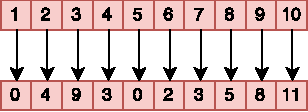
\includegraphics[scale=0.5]{images/parEvalN}
\end{center}
\end{frame}
\begin{frame}[fragile]{Basic Parallelism (2)}
\begin{lstlisting}[frame=htrbl]
parEvalN :: [a -> b] -> [a] -> [b]
\end{lstlisting}
Roadmap:
\begin{itemize}
\item Implement using existing Haskells
\begin{itemize}
\item GpH
\item ParMonad
\item Eden
\end{itemize}
\item Generalize to Arrows
\item Profit
\end{itemize}
\end{frame}

\begin{frame}[fragile]{GpH}
\begin{lstlisting}[frame=htrbl]
parEvalN :: (NFData b) => [a -> b] -> [a] -> [b]
parEvalN fs as = zipWith ($) fs as `using` parList rdeepseq
\end{lstlisting}
\begin{center}
	\includegraphics[scale=0.5]{images/parEvalNMulticore}
\end{center}
\end{frame}

\begin{frame}[fragile]{Par Monad}
\begin{lstlisting}[frame=htrbl]
parEvalN :: (NFData b) => [a -> b] -> [a] -> [b]
parEvalN fs as = runPar $ 
	(sequenceA $ map (spawnP) $ zipWith ($) fs as) >>= mapM get
\end{lstlisting}
\begin{center}
\includegraphics[scale=0.4]{images/parEvalNParMonad1}
\end{center}
\end{frame}

\begin{frame}[fragile]{Par Monad}
\begin{lstlisting}[frame=htrbl]
parEvalN :: (NFData b) => [a -> b] -> [a] -> [b]
parEvalN fs as = runPar $ 
	(sequence $ map (spawnP) $ zipWith ($) fs as) >>= mapM get
\end{lstlisting}
\begin{center}
	\includegraphics[scale=0.4]{images/parEvalNParMonad2}
\end{center}
\end{frame}

\begin{frame}[fragile]{Par Monad}
\begin{center}
	\includegraphics[scale=0.4]{images/parEvalNParMonad}
\end{center}
\end{frame}

\begin{frame}[fragile]{Eden}
\begin{lstlisting}[frame=htrbl]
parEvalN :: (Trans a, Trans b) => [a -> b] -> [a] -> [b]
parEvalN = spawnF
\end{lstlisting}
\begin{center}
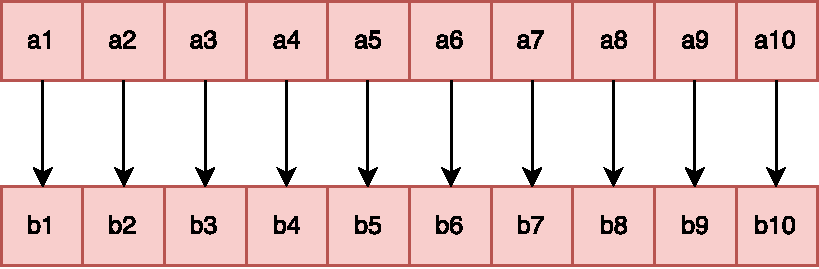
\includegraphics[scale=0.4]{images/parEvalNEden}
\end{center}
\end{frame}